% !TeX root = ../../infdesc.tex
\section{Sets}
\secbegin{secSets}
\index{set|(}

We begin by redefining the notion of a \textit{set} with a notch more precision than we provided in \Cref{chGettingStarted}. At their core, sets seem extremely simple---sets are just collections of objects---except that if not kept in check, this characterisation of a set leads to logical inconsistencies, such as the infamous \textit{Russell's paradox}.

These logical paradoxes can be overcome by restricting ourselves to working inside a \textit{universe} $\mathcal{U}$, which we consider to be a set which is so big that it contains all of the mathematical objects that we want to talk about. This is a subtle issue, which is well beyond the scope of this section, but is discussed further in \Cref{secZFC}.

\begin{definition}
\label{defSet}
\index{set}
\index{element}
\index{universal set}
\index{universe!of discourse}
A \textbf{set}\index{set} is a collection of \textbf{elements} from a specified \textbf{universe of discourse}\index{universe of discourse}. The collection of everything in the universe of discourse is called the \textbf{universal set}\index{set!universal}, denoted by $\mathcal{U}$\nindex{U}{$\mathcal{U}$}{universal set} \inlatex{mathcal\{U\}}\lindexmmc{mathcal}{$\mathcal{A}, \mathcal{B}, \dots$}.

The expression $x \in X$\nindex{in}{$\in$}{element} \inlatex{in}\lindexmmc{in}{$\in$} denotes the statement that $x$ is an element of $X$; we write $x \not \in X$ \inlatex{not\textbackslash{}in}\lindexmmc{not}{$\not\in, \not\equiv, \dots$} to mean $\neg (x \in X)$, that is that $x$ is not an element of $X$.
\end{definition}

\begin{example}
In \Cref{chGettingStarted}, we introduced five sets: the set $\mathbb{N}$ of natural numbers, the set $\mathbb{Z}$ of integers, the set $\mathbb{Q}$ of rational numbers, the set $\mathbb{R}$ of real numbers and the set $\mathbb{C}$ of complex numbers.
\end{example}

\begin{exercise}
Which of the following propositions are true, and which are false?
\[ \frac{1}{2} \in \mathbb{Z} \qquad \frac{1}{2} \in \mathbb{Q} \qquad \mathbb{Z} \in \mathbb{Q} \qquad \mathbb{Z} \in \mathcal{U} \qquad \frac{1}{2} \in \mathcal{U} \]
\hintlabel{exElementsOfSets}{%
Think about what `$a \in X$' \textit{really means}---don't let your intuition fool you.
}
\end{exercise}

We will avoid referring explicitly to the universal set $\mathcal{U}$ whenever possible, but it will always be there in the background. This is convenient because we no longer need to worry about the domain of discourse of free variables (as we did in \Cref{defPredicate}), so that we can abbreviate `$\forall x \in \mathcal{U},\, p(x)$' by `$\forall x,\, p(x)$', and `$\exists x \in \mathcal{U},\, p(x)$' by `$\exists x,\, p(x)$'.

Note that under this convention:
\begin{itemize}
\item $\forall x \in X,\, p(x)$ is logically equivalent to $\forall x,\, (x \in X \Rightarrow p(x))$; and
\item $\exists x \in X,\, p(x)$ is logically equivalent to $\exists x,\, (x \in X \wedge p(x))$.
\end{itemize}

\subsection*{Specifying a set}
One way of defining a set is simply to describe it in words, like we have done up to now. There are other, more concise ways of specifying sets, which also remove such ambiguity from the process.

\textbf{Lists.}\index{list notation}
One way is simply to provide a \textbf{list} of the elements of the set. To specify that the list denotes a set, we enclose the list with $\{$curly brackets$\}$\nindex{set}{$\{ \cdots \}$}{set notation} \inlatex{\{,\textbackslash{}\}}\lindexmmc{\{\dots\textbackslash{}\}}{$\{\dots\}$}. For example, the following is a specification of a set $X$, whose elements are the natural numbers between $0$ and $5$ (inclusive):
\[ X = \{ 0, 1, 2, 3, 4, 5 \} \]

\textbf{Implied lists.}\index{implied list notation}
Sometimes a list might be too long to write out---maybe even infinite---or the length of the list might depend on a variable. In these cases it will be convenient to use an \textbf{implied list}, in which some elements of the list are written, and the rest are left implicit by writing an ellipsis `$\dots$' \inlatex{dots}\lindexmmc{dots}{$\dots$}. For example, the statement
\[ X = \{ 1, 4, 9, \dots, n^2 \} \]
means that $X$ is the set whose elements are all the square numbers from $1$ to $n^2$, where $n$ is some number. Implied lists can be ambiguous, since they rely on the reader's ability to infer the pattern being followed, so use with caution!

\textbf{Set-builder notation.}\index{set-builder notation}
In general, implied lists can be ambiguous, so in practice they are avoided unless the implied list is very simple, such as a set of consecutive numbers like $\{3, 4, \dots, 9 \}$. In fact, many sets can't even be listed in this way.

To get around this, we can use \textit{set-builder notation}, which is a means of specifying a set in terms of the properties its elements satisfy. Given a set $X$, the set of elements of $X$ satisfying some property $p(x)$ is denoted
\[ \{ x \in X \mid p(x) \} \]
The bar `$\mid$' \inlatex{mid}\lindexmmc{mid}{$\mid$} separates the variable name from the formula that they make true---some authors use a colon instead (as in $\{ x \in X : p(x) \}$).

The set $\{ x \in X \mid p(x) \}$ is read aloud as `the set of $x \in X$ such that $p(x)$', but beware---neither the bar `$\mid$' nor the colon `$:$' mean `such that' in other contexts.

\begin{example}
\label{exSetsSpecifyUniverses}
The set of all even integers can be written in set-builder notation as
\[ \{ n \in \mathbb{Z} \mid n \text{ is even} \} \]
For comparison, the set of all even natural numbers can be written as
\[ \{ n \in \mathbb{N} \mid n \text{ is even} \} = \{ 0, 2, 4, 6, \dots \} \]
Note that $-6$ is an element of the former set but not of the latter set, since $-6$ is an integer but is not a natural number.

Note moreover that the expression
\[ \{ n \in \mathbb{Q} \mid n \text{ is even} \} \]
is meaningless, since we have not defined a notion of `evenness' for rational numbers.
\end{example}

\begin{strategy}
Let $X$ be a set and let $p(x)$ be a logical formula with free variable $x \in X$. In order to prove $a \in \{ x \in X \mid p(x) \}$, it suffices to prove $a \in X$ and that $p(a)$ is true.
\end{strategy}

\begin{exercise}
\label{exDyadicRatioal}
\index{rational number!dyadic}
A \textbf{dyadic rational} is a rational number that can be expressed as an integer divided by a power of $2$. Express the set of all dyadic rationals using set-builder notation.
\end{exercise}

An alternate form of set-builder notation uses an expression involving one or more variables to the left of the vertical bar, and the range of the variable(s) to the right. The elements of the set are then the values of the expression as the variable(s) vary as indicated---that is:
\[ \{ \mathsf{expr}(x) \mid x \in X \} \text{ is defined to mean } \{ y \mid \exists x \in X,\, y = \mathsf{expr}(x) \} \]
where $\mathsf{expr}(x)$ is the expression in question.

\begin{example}
The expression $\{ 3k+2 \mid k \in \mathbb{Z} \}$ denotes the set of all integers of the form $3k+2$, where $k \in \mathbb{Z}$. It is shorthand for $\{ n \in \mathbb{Z} \mid \exists k \in \mathbb{Z},\, n=3k+2 \}$. In implied list notation, we could write this set as $\{ \dots, {-4}, {-1}, 2, 5, 8, \dots \}$.
\end{example}

\begin{exercise}
Express the set of dyadic rationals (defined in \Cref{exDyadicRatioal}) in this alternate form of set-builder notation.
\end{exercise}

Set-builder notation is useful for defining sets based on the properties they satisfy, as in \Cref{defBracketN,defIntervals} below.

\begin{restatable}{definition}{RSdefBracketN}
\label{defBracketN}
Let $n \in \mathbb{N}$. The set $[n]$ is defined by $[n] = \{ k \in \mathbb{N} \mid 1 \le k \le n \}$.
\end{restatable}

\begin{example}
\label{exBracketN}
In implied list notation, $[n] = \{ 1, 2, \dots, n \}$. For example, $[4] = \{ 1, 2, 3, 4 \}$. Note that $[0]$ has no elements (it is \textit{empty}---see \Cref{defInhabited}), since there are no natural numbers $k$ satisfying the inequality $1 \le k \le 0$.
\end{example}

While not particularly interesting yet, sets of the form $[n]$ will be fundamental throughout \Cref{chCombinatorics}, as they are used to define the notion of a \textit{finite set}, as well as the \textit{size} of a finite set.

Intervals are particular subsets of $\mathbb{R}$ that are ubiquitous in mathematics, particularly in analysis and topology.

\begin{definition}[Intervals of the real line]
\label{defIntervals}
\index{interval!open}
\index{interval!closed}
\index{interval!half-open}
\index{open!interval}
\index{closed!interval}
\nindex{abint1}{$(a,b)$}{open interval}
\nindex{abint2}{$[a,b]$}{closed interval}
\nindex{abint3}{$(a,b]$}{half-open interval}
\nindex{abint4}{$[a,b)$}{half-open interval}
\nindex{abint5}{$(-\infty,a)$}{unbounded interval}
\nindex{abint6}{$(a,\infty)$}{unbounded interval}
Let $a,b \in \mathbb{R}$. The \textbf{open interval} $(a,b)$, the \textbf{closed interval} $[a,b]$, and the \textbf{half-open intervals} $[a,b)$ and $(a,b]$ from $a$ to $b$ are defined by
\begin{align*}
\hspace{35pt} (a,b) &= \{ x \in \mathbb{R} \mid a < x < b \}
&
(a,b] &= \{ x \in \mathbb{R} \mid a < x \le b \} 
\\
\hspace{35pt} [a,b) &= \{ x \in \mathbb{R} \mid a \le x < b \}
&
[a,b] &= \{ x \in \mathbb{R} \mid a \le x \le b \}
\end{align*}
We further define the \textbf{unbounded intervals} $(-\infty, a)$, $(-\infty, a]$, $[a, \infty)$ and $(a, \infty)$ \inlatex{infty}\lindexmmc{infty}{$\infty$} by
\begin{align*}
\hspace{35pt} (-\infty,a) &= \{ x \in \mathbb{R} \mid x < a \}
&
(a,\infty) &= \{ x \in \mathbb{R} \mid x > a \}
\\
\hspace{35pt} (-\infty, a] &= \{ x \in \mathbb{R} \mid x \le a \} 
&
[a,\infty) &= \{ x \in \mathbb{R} \mid x \ge a \}
\end{align*}
\end{definition}

\begin{example}
The following illustration depicts the open interval $(-2,5)$.

\vspace{-10pt}
\begin{center}
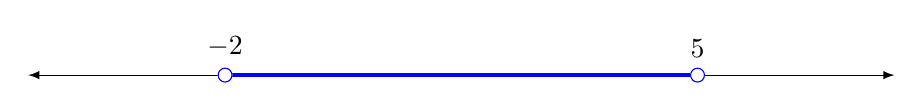
\begin{tikzpicture}
\draw[latex-latex] (-5.5,0) -- (5.5,0);
\draw[line width=1.5pt, color=blue] (-3,0) -- (3,0);
\filldraw[white](-3,0)circle[radius=2.5pt];
\draw[blue](-3,0)circle[radius=2.5pt];
\filldraw[white](3,0)circle[radius=2.5pt];
\draw[blue](3,0)circle[radius=2.5pt];
\node[at={(-3,3pt)},above]{$-2$};
\node[at={(3,3pt)},above]{$5$};
\end{tikzpicture}
\end{center}
The hollow circles $\circ$ indicate that the endpoints are not included in the interval.
\end{example}

Be warned that the use of the symbol $\infty$ is misleading, since it suggests that the symbol $\infty$ on its own has a specific meaning (or, worse, that it refers to a real number). It doesn't---it is just a symbol that suggests unboundedness of the interval in question. A less misleading way of writing $[a, \infty)$, for instance, might be $[a, {\to})$ or $\mathbb{R}^{\ge a}$; however, $[a,\infty)$ is standard, so it is what we will write.

\begin{exercise}
For each of the following illustrations, find the interval that it depicts. A filled circle $\bullet$ indicates that an end-point is included in the interval, whereas a hollow circle $\circ$ indicates that an end-point is not included in the interval.

\begin{enumerate}[(a)]
\item
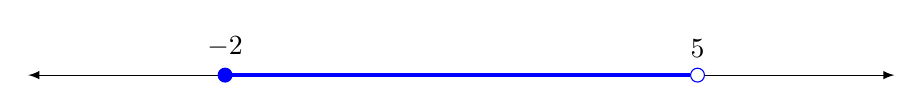
\begin{tikzpicture}
\draw[latex-latex] (-5.5,0) -- (5.5,0);
\draw[line width=1.5pt, color=blue] (-3,0) -- (3,0);
\filldraw[blue](-3,0)circle[radius=2.5pt];
\filldraw[white](3,0)circle[radius=2.5pt];
\draw[blue](3,0)circle[radius=2.5pt];
\node[at={(-3,3pt)},above]{$-2$};
\node[at={(3,3pt)},above]{$5$};
\end{tikzpicture}

\item
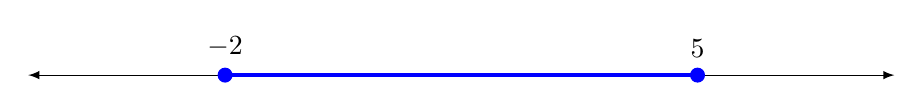
\begin{tikzpicture}
\draw[latex-latex] (-5.5,0) -- (5.5,0);
\draw[line width=1.5pt, color=blue] (-3,0) -- (3,0);
\filldraw[blue](-3,0)circle[radius=2.5pt];
\filldraw[blue](3,0)circle[radius=2.5pt];
\node[at={(-3,3pt)},above]{$-2$};
\node[at={(3,3pt)},above]{$5$};
\end{tikzpicture}


\item
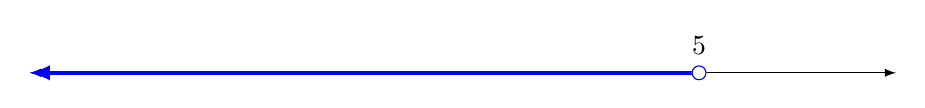
\begin{tikzpicture}
\draw[latex-latex] (-5.5,0) -- (5.5,0);
\draw[latex-, line width=1.5pt, color=blue] (-5.5,0) -- (3,0);
\filldraw[white](3,0)circle[radius=2.5pt];
\draw[blue](3,0)circle[radius=2.5pt];
\node[at={(3,3pt)},above]{$5$};
\end{tikzpicture}

\item 
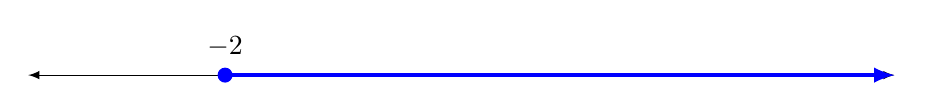
\begin{tikzpicture}
\draw[latex-latex] (-5.5,0) -- (5.5,0);
\draw[-latex, line width=1.5pt, color=blue] (-3,0) -- (5.5,0);
\filldraw[blue](-3,0)circle[radius=2.5pt];
\node[at={(-3,3pt)},above]{$-2$};
\end{tikzpicture}
\end{enumerate}
\end{exercise}

\subsection*{Subsets}

It is often the case that everything that is also an element of one set is an element of another set. For example, every integer is a rational number; that is
\[ \forall n \in \mathbb{Z},\, n \in \mathbb{Q} \]
We can say this more concisely by saying that $\mathbb{Z}$ is a \textit{subset} of $\mathbb{Q}$.

\begin{definition}
\label{defSubset}
\index{subset}
Let $X$ be a set. A \textbf{subset} of $X$ is a set $U$ such that
\[ \forall a,\, (a \in U \Rightarrow a \in X) \]
We write $U \subseteq X$\nindex{subset}{$\subseteq$}{subset} \inlatex{subseteq}\lindexmmc{subseteq}{$\subseteq$} for the assertion that $U$ is a subset of $X$.

Additionally, the notation $U \nsubseteq X$ \inlatex{nsubseteq}\lindexmmc{nsubseteq}{$\nsubseteq$} means that $U$ is not a subset of $X$, and the notation $U \subsetneqq X$ \inlatex{subsetneqq}\lindexmmc{subsetneqq}{$\subsetneqq$} means that $U$ is a \textbf{proper subset} of $X$, that is a subset of $X$ that is not equal to $X$.
\end{definition}

\begin{strategy}[Proving a subset containment]
In order to prove that a set $U$ is a subset of a set $X$, it suffices to take an arbitrary element $a \in U$ and prove that $a \in X$.
\end{strategy}

\begin{example}
Every set is a subset of itself---that is, $X \subseteq X$ for all sets $X$. The proof of this is extremely simple: we must prove $\forall x \in X,\, x \in X$. But then this is trivial: let $x \in X$, then $x \in X$ by assumption. Done!
\end{example}

\begin{example}
Let $a,b,c,d \in \mathbb{R}$ with $a<c<d<b$. Then $[c,d] \subseteq (a,b)$. Indeed, let $x \in [c,d]$. Then $c \le x \le d$. But then
\[ a < c \le x \le d < b \quad \Rightarrow \quad a < x < b \]
so that $[c,d] \subseteq (a,b)$, as required.
\end{example}

\begin{exercise}
Let $a,b,c,d \in \mathbb{R}$ with $a<b$ and $c<d$. Prove that $[a,b) \subseteq (c,d]$ if and only if $a > c$ and $b \le d$.
\end{exercise}

\begin{example}
The number sets from \Cref{chGettingStarted} are related by the following chain of subset inclusions.
\[ \mathbb{N} \subseteq \mathbb{Z} \subseteq \mathbb{Q} \subseteq \mathbb{R} \subseteq \mathbb{C} \]
\end{example}

The following proposition proves a property of subsethood known as \textit{transitivity}---we'll revisit this property in \Cref{secRelations}.

\begin{proposition}
\label{propSubsetTransitive}
Let $X,Y,Z$ be sets. If $X \subseteq Y$ and $Y \subseteq Z$, then $X \subseteq Z$.
\end{proposition}

\begin{cproof}
Suppose that $X \subseteq Y$ and $Y \subseteq Z$. We need to prove $X \subseteq Z$.

So let $a \in X$. Since $X \subseteq Y$, it follows from \Cref{defSubset} that $a \in Y$; and since $Y \subseteq Z$, it follows again from \Cref{defSubset} that $a \in Z$.

Hence $X \subseteq Z$, as required.
\end{cproof}

\subsection*{Set equality}

This section is all about defining sets, comparing sets, and building new sets from old, and so to make much more progress, we first need to establish what we mean when we say that two sets are \textit{equal}.

\begin{discussion}
\label{dscSetEquality}
Let $X$ and $Y$ be sets. What should it mean to say that $X$ and $Y$ are equal? Try to provide a precise definition of equality of sets before reading on.
\end{discussion}

There are different possible notions of `sameness' for sets: we might want to say that two sets $X$ and $Y$ are equal when they have quite literally the same definition; or we might want to say that $X$ and $Y$ are equal when they contain the same objects as elements. For instance, suppose $X$ is `the set of all odd natural numbers' and $Y$ is `the set of all integers that are differences of consecutive perfect squares'---in this case, the first of these characterisations of equality might lead us to say $X \ne Y$, whereas the second would lead us to say $X = Y$.

Clearly, we have to state our terms at some point. And that point is now.

\begin{axiom}[Set extensionality]
\label{axSetEquality}
\index{set equality}
\index{extensionality}
Let $X$ and $Y$ be sets. Then $X=Y$ if and only if $\forall a,\, (a \in X \Leftrightarrow a \in Y)$, or equivalently, if $X \subseteq Y$ and $Y \subseteq X$.
\end{axiom}

This characterisation of set equality suggests the following strategy for proving that two sets are equal.

\begin{strategy}[Proof by double containment]
In order to prove that a set $X$ is equal to a set $Y$, it suffices to:
\begin{itemize}
\item Prove $X \subseteq Y$, i.e.\ let $a \in X$ be an arbitrary element, and derive $a \in Y$; and then
\item Prove $X \supseteq Y$, i.e.\ let $a \in Y$ be an arbitrary element, and derive $a \in X$.
\end{itemize}
We often write `($\subseteq$)' and `($\supseteq$)' to indicate the direction of the containment being proved.
\end{strategy}

\begin{example}
\label{exPositiveNegativeSetBuilderNotation}
We prove that $\{ x \in \mathbb{R} \mid x^2 \le 1 \} = [-1,1]$ by double containment.
\begin{itemize}
\item ($\subseteq$) Let $a \in \{ x \in \mathbb{R} \mid x^2 \le 1 \}$. Then $a \in \mathbb{R}$ and $a^2 \le 1$, so that $(1-a)(1+a) = 1-a^2 \ge 0$. It follows that either:
\begin{itemize}
\item $1-a \ge 0$ and $1+a \ge 0$, in which case $a \le 1$ and $a \ge -1$, so that $a \in [-1,1]$.
\item $1-a \le 0$ and $1+a \le 0$, in which case $a \ge 1$ and $a \le -1$, which is a contradiction since $-1 < 1$.
\end{itemize}
So we must have $a \in [-1,1]$, as required.

\item ($\supseteq$) Let $a \in [-1,1]$. Then $-1 \le a \le 1$, so $|a| \le 1$, and hence $a^2 = |a|^2 \le 1$, so that $a \in \{ x \in \mathbb{R} \mid x^2 \le 1 \}$, as required.
\end{itemize}
\end{example}

\begin{exercise}
Prove that $\{ x \in \mathbb{R} \mid x^2 < x \} = (0,1)$.
\end{exercise}

The set extensionality axiom has the consequence that sets are independent of the order in which their elements appear in list notation, and they are independent of how many times a single element is written---that is, an element of a set is only `counted' once, even if it appears multiple times in list notation. This is illustrated in the following exercise.

\begin{exercise}
Prove by double containment that $\{ 0, 1 \} = \{ 1, 0 \}$ and $\{ 0, 0 \} = \{ 0 \}$.
\end{exercise}

\subsection*{Inhabitation and emptiness}

Another fundamental example of a set is the \textit{empty set}, which is the set with no elements. But we have to be slightly careful about how we use the word `the', since it implies \textit{uniqueness}, and we don't know (yet) that two sets with no elements are necessarily equal. So first we will define what it means for a set to be empty, and then we'll show that there is exactly one empty set.

\begin{definition}
\label{defInhabited}
\label{defEmptyProperty}
\index{empty set}
\index{set!empty}
\index{inhabited set}
\index{set!inhabited}
A set $X$ is \textbf{inhabited} (or \textbf{nonempty}) if it has at least one element; otherwise, it is \textbf{empty}.
\end{definition}

The assertion that $X$ is inhabited is equivalent to the logical formula $\exists a,\, a \in X$, and the assertion that $X$ is empty is equivalent to the logical formula $\neg \exists a,\, a \in X$. This suggests the following strategy for proving that a set is inhabited, or that it is empty.

\begin{strategy}[Proving that a set is inhabited or empty]
In order to prove a set $X$ is inhabited, it suffices to exhibit an element. In order to prove a set $X$ is empty, assume that $X$ is inhabited---that is, that there is some element $a \in X$---and derive a contradiction.
\end{strategy}

In other texts, the term \textit{nonempty} is more common than \textit{inhabited}, but there are reasons to prefer latter. Indeed, the statement `$X$ is non-empty' translates more directly to $\neg(\neg \exists a,\, a \in X)$, which has an unnecessary double-negative and suggests a proof of inhabitation by contradiction. For this reason, we use the term \textit{inhabited} in this book.

Emptiness may seem like a trivial condition---and it is---but owing to its canonicity, it arises all over the place.

\begin{example}
The set $\{ x \in \mathbb{R} \mid x^2 = 2 \}$ is inhabited since, for example $\sqrt{2} \in \mathbb{R}$ and $\sqrt{2}^2 = 2$. However, the set $\{ x \in \mathbb{Q} \mid x^2 = 2 \}$ is empty since, if it were inhabited, then there would be a rational number $x$ such that $x^2 = 2$, contrary to \Cref{propSqrt2IrrationalPreliminary}.
\end{example}

\begin{example}
We observed in \Cref{exBracketN} that the set $[0]$ is empty; here's a more formal proof. Towards a contradiction, suppose $[0]$ is inhabited. Then there is some $k \in \mathbb{N}$ such that $1 \le k \le 0$. It follows that $1 \le 0$, which contradicts the fact that $0<1$. Hence $[0]$ is empty, after all.
\end{example}

\begin{exercise}
Let $a,b \in \mathbb{R}$. Prove that $[a,b]$ is empty if and only if $a > b$, and that $(a,b)$ is empty if and only if $a \ge b$.
\end{exercise}

The next exercise is a logical technicality, which is counterintuitive for the same reason that makes the principle of explosion (\Cref{axPrincipleOfExplosion}) difficult to grasp. However, it is extremely useful for proving facts about the empty set, as we will see soon in \Cref{thmEmptySetIsUnique}.

\begin{exercise}
Let $E$ be an empty set and let $p(x)$ be a predicate with one free variable $x$ with domain of discourse $E$. Show that the proposition $\forall x \in E,\, p(x)$ is true, and that the proposition $\exists x \in E,\, p(x)$ is false. What does the proposition $\forall x \in E,\, x \ne x$ mean in English? Is it true?
\hintlabel{exEverythingIsTrueOfElementsOfEmptySet}{%
Recall from the beginning of \Cref{secSets} that $\forall x \in X,\, p(x)$ is equivalent to $\forall x,\, (x \in X \Rightarrow p(x))$ and $\exists x \in X,\, p(x)$ is equivalent to $\exists x,\, (x \in X \wedge p(x))$. What can be said about the truth value of $x \in E$ when $E$ is empty?
}
\end{exercise}

Thanks to the axiom of extensionality (\Cref{axSetEquality}), any two empty sets must be equal since they both contain the same elements---namely, no elements at all! This is made formal in the following theorem.

\begin{theorem}
\label{thmEmptySetIsUnique}
Let $E$ and $E'$ be sets. If $E$ and $E'$ are empty, then $E=E'$.
\end{theorem}
\begin{proof}
Suppose that $E$ and $E'$ are empty. The assertion that $E=E'$ is equivalent to
\[ (\forall a \in E,\, a \in E') \wedge (\forall a \in E',\, a \in E) \]
But $\forall a \in E,\, a \in E'$ and $\forall a \in E',\, a \in E$ are both true by \Cref{exEverythingIsTrueOfElementsOfEmptySet} since $E$ and $E'$ are empty. So $E=E'$, as claimed.
\end{proof}

Knowing that there is one and only one empty set means that we may now make the following definition, without worrying about whether the word `the' is problematic.

\begin{definition}
\label{defEmptySet}
\nindex{O}{$\varnothing$}{empty set}
\index{empty set}
\index{set!empty}
The \textbf{empty set} (also known as the \textbf{null set}) is the set with no elements, and is denoted by $\varnothing$ \inlatex{varnothing}\lindexmmc{varnothing}{$\varnothing$}.
\end{definition}

Some authors write $\{ \}$ instead of $\varnothing$, since $\{ \}$ is simply the empty set expressed in list notation.

\begin{exercise}
\label{exEmptySetSubsetOfEverySet}
Let $X$ be a set. Prove that $\varnothing \subseteq X$.
\end{exercise}

\subsection*{Power sets}

\begin{definition}
\label{defPowerSet}
\index{power set}
Let $X$ be a set. The \textbf{power set} of $X$, written $\mathcal{P}(X)$\nindex{PX}{$\mathcal{P}(X)$}{power set} \inlatex{mathcal\{P\}}\lindexmmc{mathcal}{$\mathcal{A}, \mathcal{B}, \dots$}, is the set of all subsets of $X$.
\end{definition}

\begin{example}
There are four subsets of $\{ 1, 2 \}$, namely
\[ \varnothing, \quad \{ 1 \}, \quad \{ 2 \}, \quad \{ 1, 2 \} \]
so $\mathcal{P}(X) = \{\varnothing, \{ 1 \}, \{ 2 \}, \{ 1, 2 \}\}$.
\end{example}

\begin{exercise}
Write out the elements of $\mathcal{P}(\{1, 2, 3\})$.
\end{exercise}

\begin{exercise}
Let $X$ be a set. Show that $\varnothing \in \mathcal{P}(X)$ and $X \in \mathcal{P}(X)$.
\end{exercise}

\begin{exercise}
Write out the elements of $\mathcal{P}(\varnothing)$, $\mathcal{P}(\mathcal{P}(\varnothing))$ and $\mathcal{P}(\mathcal{P}(\mathcal{P}(\varnothing)))$.
\end{exercise}

Power sets are often a point of confusion because they bring the property of being a \textit{subset} of one set to that of being an \textit{element} of another, in the sense that for all sets $U$ and $X$ we have
\[ U \subseteq X \quad \Leftrightarrow \quad U \in \mathcal{P}(X) \]
This distinction looks easy to grasp, but when the sets $U$ and $X$ look alike, it's easy to fall into various traps. Here's a simple example.

\begin{example}
It is true that $\varnothing \subseteq \varnothing$, but false that $\varnothing \in \varnothing$. Indeed,
\begin{itemize}
\item $\varnothing \subseteq \varnothing$ means $\forall x \in \varnothing,\, x \in \varnothing$; but propositions of the form $\forall x \in \varnothing,\, p(x)$ are always true, as discussed in \Cref{exEverythingIsTrueOfElementsOfEmptySet}.
\item The empty set has no elements; if $\varnothing \in \varnothing$ were true, it would mean that $\varnothing$ had an element (that element being $\varnothing$). So it must be the case that $\varnothing \not \in \varnothing$.
\end{itemize}
\end{example}

The following exercise is intended to help you overcome similar potential kinds of confusion by means of practice. Try to think precisely about what the definitions involved are.

\begin{exercise}
Determine, with proof, whether or not each of the following statements is true.
\begin{enumerate}[(a)]
\item $\mathcal{P}(\varnothing) \in \mathcal{P}(\mathcal{P}(\varnothing))$;
\item $\varnothing \in \{ \{ \varnothing \} \}$;
\item $\{ \varnothing \} \in \{ \{ \varnothing \} \}$;
\item $\mathcal{P}(\mathcal{P}(\varnothing)) \in \{ \varnothing, \{ \varnothing, \{ \varnothing \} \} \}$.
\end{enumerate}
Repeat the exercise with all instances of `$\in$' replaced by `$\subseteq$'.
\end{exercise}

\begin{tldr}{secSets}

\subsubsection*{Sets and subsets}

\begin{tldrlist}
\tldritem{defSet} A \textit{set} is a collection of objects (called \textit{elements}) from a fixed \textit{universe of discourse} $\mathcal{U}$; we write $x \in X$ to mean that $x$ is an element of the set $X$. Sets can be specified by (explicitly or implicitly) listing their elements $\{ x_1, x_2, \dots, x_n, \dots \}$, or by using \textit{set-builder notation} $\{ x \in X \mid p(x) \}$.
\tldritem{defSubset} A set $U$ is a \textit{subset} of a set $X$, written $U \subseteq X$, if $\forall a,\, (a \in U \Rightarrow a \in X)$. To prove that $U \subseteq X$, it suffices to introduce a variable $a$, assume that $a \in U$, and derive $a \in X$.
\tldritem{axSetEquality} Sets $X$ and $Y$ are equal if and only if $\forall a,\, (a \in X \Leftrightarrow a \in Y)$. In order to prove that $X = Y$, it suffices to prove separately that $X \subseteq Y$ and $Y \subseteq X$---this method is called \textit{double containment}.
\end{tldrlist}

\subsubsection*{Inhabitation and emptiness}

\begin{tldrlist}
\tldritem{defInhabited} A set $X$ is \textit{inhabited} if it has at least one element; otherwise, it is \textit{empty}.
\tldritem{thmEmptySetIsUnique} There is a unique empty set, denoted by $\varnothing$ or $\{ \}$.
\end{tldrlist}

\subsubsection*{Power sets}
\begin{tldrlist}
\tldritem{defPowerSet} The \textit{power set} of a set $X$ is the set of all subsets of $X$.
\end{tldrlist}
\end{tldr}